\documentclass[conference]{IEEEtran}
\IEEEoverridecommandlockouts
\usepackage{amsmath,amssymb}
\usepackage{graphicx}
\usepackage{booktabs}
\usepackage{xcolor}
\usepackage[hidelinks]{hyperref}
\usepackage{url}
\renewcommand{\ttdefault}{lmtt}
\graphicspath{{../figures/}}
\newcommand{\figsize}{\linewidth}

\begin{document}

\title{When Does Memory Break? Sharpness, Capacity and False Memories in Classical, Dense and Modern Hopfield Networks}

\author{\IEEEauthorblockN{Soham Chatterjee (2023101092)}
\IEEEauthorblockA{Introduction to Neural and Cognitive Modelling, 2026 --- Final project report\\
Code: \url{https://github.com/GrandsonOfBuddha/modern-hopfield-memory}}}

\maketitle

\begin{abstract}
The classical Hopfield network stores only about $0.14N$ memories in $N$ neurons and produces spurious ``false memories''. Dense associative memory and the modern (softmax) Hopfield network claim to remove this limit. I compare the three models along a single \emph{sharpness} dial (linear, polynomial power $n$, inverse temperature $\beta$) on random patterns, MNIST digits and GloVe word vectors, using identical memories and cues. I reproduce the $0.14N$ limit, the $N^{n-1}$ scaling of dense memories and the exponential capacity of the modern network. On correlated data (MNIST, mean pairwise cosine 0.66) the classical network fails with only 10 stored digits, while a sharp modern network recalls noisy digits as well as a nearest-neighbour lookup up to 20\,000 digits. Counting synapses changes the picture: at an equal synapse budget the modern network stores only $\approx$3.6$\times$ more memories, not exponentially more. Hetero-association with unrelated pairs is \emph{easier} than auto-association, contrary to my prediction. Finally, a modern network on GloVe vectors reproduces the DRM false-memory effect, including its growth with list length, at low $\beta$ ($\beta\approx3$ gives 48\% false recall vs 46\% in humans), and sharp retrieval ($\beta\ge10$) removes it.
\end{abstract}

\section{Aim of the Modelling Exercise}
To test, with one common set of tasks and cues, (\textbf{Q1}) how much the modern Hopfield networks can store and at what cost in synapses; (\textbf{Q2}) whether they still make false memories when memories are similar, as people do in the DRM paradigm; and (\textbf{Q3}) whether recalling a paired partner (hetero-association) is harder than restoring the item itself (auto-association). The unifying hypothesis is that one parameter, the \emph{sharpness} with which a cue selects the best-matching memory, controls all three.

\section{Introduction and Motivation}
\textbf{Classical model.} The Hopfield network~\cite{hopfield82} stores binary patterns $\boldsymbol\xi^\mu\in\{\pm1\}^N$ in Hebbian weights $W=\frac1N\sum_\mu\boldsymbol\xi^\mu\boldsymbol\xi^{\mu\top}$; a damaged cue descends the energy $E=-\frac12\boldsymbol\sigma^\top W\boldsymbol\sigma$ to the nearest attractor. Above $K\approx0.138N$ memories recall collapses~\cite{ags85}, and mixtures of memories become stable spurious states. Correlated patterns (real images, related words) reduce capacity much further.

\textbf{Variations studied.} \emph{Dense associative memory}~\cite{krotov16} replaces the quadratic energy by $E=-\sum_\mu F(\boldsymbol\xi^{\mu\top}\boldsymbol\sigma)$ with $F(x)=x^n$; capacity grows as $N^{n-1}$. The \emph{modern Hopfield network}~\cite{ramsauer21} uses continuous states, the energy $E=-\beta^{-1}\log\sum_\mu e^{\beta\,\mathbf{x}_\mu^\top\boldsymbol\xi}+\frac12\|\boldsymbol\xi\|^2$ and the one-step update $\boldsymbol\xi^{\rm new}=X^\top\mathrm{softmax}(\beta X\boldsymbol\xi)$, which is transformer attention; its capacity is exponential in $N$~\cite{demircigil17,ramsauer21}. Millidge et al.~\cite{millidge22} showed that all three are one computation, \emph{similarity $\rightarrow$ separation $\rightarrow$ projection}, differing only in the separation function (linear, polynomial, softmax). Krotov \& Hopfield~\cite{krotov21} showed the dense/modern models can be built from ordinary neurons with one hidden ``memory neuron'' per pattern, which makes their synaptic cost countable.

\textbf{Cognitive motivation.} After studying \emph{bed, rest, tired, dream}\ldots{} people often recall the unstudied lure \emph{sleep} (DRM paradigm~\cite{roediger95}); the lure is recalled with probability 0.46 on average across 36 lists~\cite{stadler99}, and this rate grows with the number of studied associates~\cite{robinson97}. Global-matching models such as MINERVA~2, whose activation is the \emph{cube} of similarity (a dense memory with $n=3$), explain false \emph{recognition} by summed similarity~\cite{arndt98}. Whether the newer, sharper Hopfield models still produce such errors, and how sharpness trades capacity against generalisation, has not, to my knowledge, been tested on the DRM lists. Paired-associate learning~\cite{nelson04} motivates the auto/hetero comparison.

\section{Methods}
\subsection{Models}
All binary models update neurons \emph{asynchronously} in random order until no neuron changes (max.\ 30 sweeps). \textbf{Classical:} $\sigma_i\leftarrow\mathrm{sgn}(\sum_{j\ne i}W_{ij}\sigma_j)$. \textbf{Dense ($n$):} $\sigma_i\leftarrow\mathrm{sgn}\sum_\mu[F(\xi^\mu_i+m'_\mu)-F(-\xi^\mu_i+m'_\mu)]$, $m'_\mu=\sum_{j\ne i}\xi^\mu_j\sigma_j$, with $F(x)=x^n$; $n=2$ is exactly the classical network (verified by a unit test). \textbf{Modern ($\beta$):} patterns and state are scaled to unit length so $X\boldsymbol\xi$ are cosines and $\beta$ means the same on every data set; the update is iterated to convergence ($\le$10 steps, tolerance $10^{-6}$). \textbf{Hetero-association} replaces the projection: output $=\mathrm{sgn}(Z^\top g(X\mathbf{c}))$ with $g$ linear (classical, i.e.\ the linear associator $W=Z^\top X/N$), $g=F'$ (dense) or softmax (modern, unsigned), for partner patterns $Z$. \textbf{Nearest neighbour} (the $\beta\to\infty$ limit) is a reference ceiling. Fig.~\ref{fig:sharp} shows the dial.

\begin{figure}[t]
\centering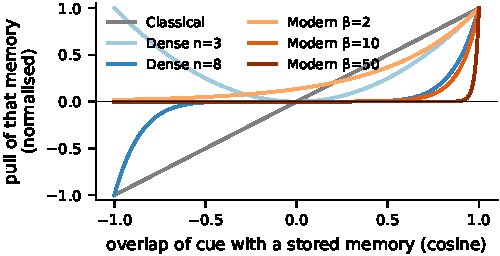
\includegraphics[width=\figsize]{fig1_sharpness.pdf}
\caption{The sharpness dial: how strongly a stored memory pulls the state as a function of its overlap with the cue (separation function~\cite{millidge22}).}
\label{fig:sharp}
\end{figure}

\subsection{Data and cues}
\emph{Random:} i.i.d.\ $\pm1$ patterns, $N\in\{8,\ldots,256\}$; cue = 10\% of bits flipped. \emph{MNIST}~\cite{lecun98}: training digits binarised at 0.5 ($N=784$), sampled class-balanced; cues have 20\% pixels flipped, or the bottom half hidden (set to background). \emph{Words:} 100-d GloVe vectors~\cite{pennington14} (6B tokens) for the 20\,000 most frequent words plus all DRM words. For binary models a word is coded as $\mathrm{sgn}(R(\mathbf{v}-\bar{\mathbf{v}}))$ with a Gaussian $R\in\mathbb{R}^{512\times100}$ (random-hyperplane hashing~\cite{charikar02} preserves angles); cues flip 20\% of the bits. Related pairs pair a word with its nearest GloVe neighbour (e.g.\ \emph{exact--precise}; code cosine 0.54 vs 0.02 for random pairs); unrelated pairs re-shuffle the same targets. \emph{DRM:} 31 lists of 15 associates~\cite{roediger95,stadler99}.

\subsection{Experiments and parameters}
\textbf{E1 Capacity.} Classical, dense $n\in\{3,4\}$, modern $\beta\in\{8,32,128\}$; $K$ on a geometric grid up to $2^{15}$ (dense) or $2^{17}$ (modern). \textbf{E2 MNIST.} Classical, dense $n\in\{4,8,16\}$, modern $\beta\in\{30,100,300,1000\}$, $K\in[10,20\,000]$; failures are labelled \emph{mix-up} (the state is a different stored digit, same or other class) or \emph{blend} (no stored digit within cosine 0.95). \textbf{E3 Words.} $N=512$, $K\in[8,4096]$; tasks: auto (recurrent), auto (one step), hetero related, hetero unrelated; dense $n\in\{3,4\}$, modern $\beta\in\{10,30,100\}$. \textbf{E4 DRM.} Store the first $k\in\{3,6,9,12,15\}$ associates of a list; \emph{free recall} starts the network from a random state, lets it settle and reads out the nearest of the 20\,000 lexicon words (studied word = veridical, lure = false recall). \emph{Recognition} ($k=15$) compares the familiarity $-E$ of the lure with that of each studied word. Modern networks are run on the GloVe vectors ($\beta\in\{1,\ldots,100\}$) and, as a control, on the binary codes; 31 lists $\times$ 3 random codings $\times$ 40 starts. \textbf{E5 Synapses.} Classical: $N(N{-}1)/2$ synapses. Dense/modern in the two-layer form~\cite{krotov21}: $NK$ synapses. Matched-budget test: give every model $S=N(N{-}1)/2$ synapses, i.e.\ $(N{-}1)/2$ memory neurons, and store that many patterns.

\textbf{Metrics.} A trial succeeds if the final state's most similar stored memory is the target with cosine $\ge0.95$. Capacity = largest $K$ (log-interpolated) recalled in $\ge90\%$ of trials. Every point uses 20 independent pattern sets $\times$ 5--10 cues (100--200 trials); all models see identical memories and cues.

\section{Results}
\subsection{Capacity and its cost (Q1)}
\begin{figure*}[t]
\centering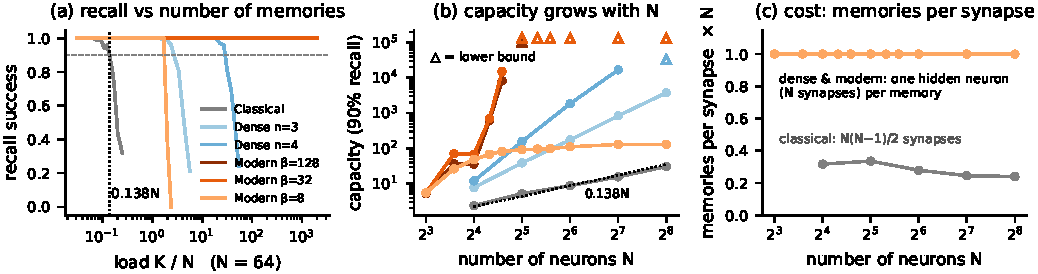
\includegraphics[width=\textwidth]{fig2_capacity.pdf}
\caption{E1/E5, random patterns, 10\% noisy cues. (a) Recall vs load at $N=64$. (b) Capacity vs $N$ (colours as in (a)); open triangles are lower bounds (never failed on the tested grid). (c) Memories per synapse $\times N$: the two-layer modern/dense network always pays $N$ synapses per memory.}
\label{fig:cap}
\end{figure*}
The classical network reaches $K/N=0.12$ at $N=256$ (theory 0.138 for zero-noise cues), and capacity grows linearly with $N$ (Fig.~\ref{fig:cap}b, slope 0.85; finite-size effects lower it below 1). Dense memories scale polynomially: fitted log--log slopes 2.2 and 3.4 for $n=3,4$, close to the predicted $n-1$~\cite{krotov16}. For the modern network capacity exceeded the largest tested $K$ ($2^{17}$) already at $N\ge32$ for $\beta\ge32$, and below that it grows exponentially ($\ln K\approx0.45N$ for $N\le24$ in $\log K$ per neuron). A new observation is that a \emph{blunt} modern network ($\beta=8$) saturates at $\approx$130 memories regardless of $N$: when $\beta$ is too small the softmax cannot single out one of many memories, so sharpness, not size, sets the limit.

Counting synapses removes most of the advantage (Fig.~\ref{fig:cap}c). The classical network stores $\approx0.12N$ memories in $N^2/2$ synapses ($\approx0.24/N$ per synapse); a two-layer modern network uses exactly $N$ synapses per memory ($1/N$), a constant $\approx$4$\times$ better. In the matched-budget test the dense and modern networks recalled all $(N{-}1)/2$ patterns (success 1.00 for $N=64$--512) while the classical network recalled none (0.00). Exponential capacity is therefore capacity \emph{per feature neuron}; per synapse the gain is a constant factor.

\subsection{Handwritten digits (Q1, Q2)}
\begin{figure*}[t]
\centering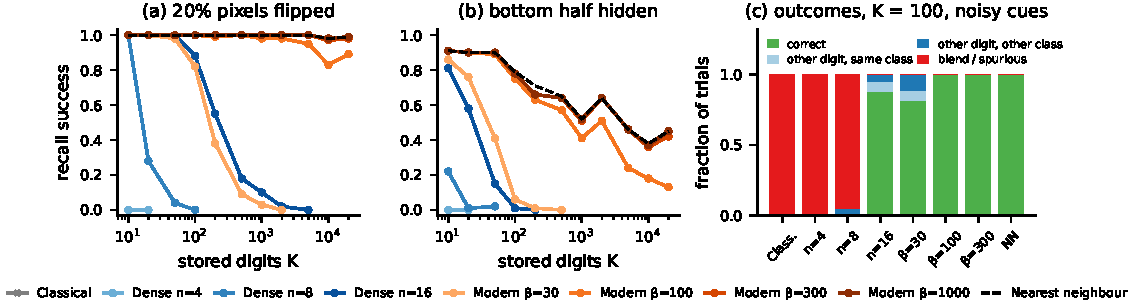
\includegraphics[width=\textwidth]{fig3_mnist.pdf}
\caption{E2, MNIST ($N=784$). (a) Noisy cues and (b) half-occluded cues: fraction recalled correctly vs number of stored digits. (c) What happens at $K=100$ (noisy cues).}
\label{fig:mnist}
\end{figure*}
\begin{figure}[t]
\centering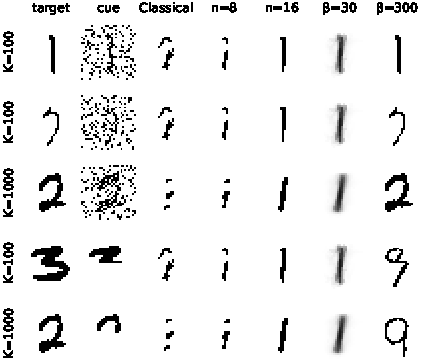
\includegraphics[width=0.93\linewidth]{fig4_mnist_examples.pdf}
\caption{Example recalls (rows: noisy cues at $K=100$/1000, occluded cues at $K=100$/1000). Blunt models all fall into the same ``average digit''; the sharp modern network ($\beta=300$) restores the digit, or recalls another real digit (3$\to$9) when the cue is ambiguous.}
\label{fig:ex}
\end{figure}
MNIST digits are highly correlated (mean pairwise cosine 0.66), which breaks the blunt models completely (Fig.~\ref{fig:mnist}): the classical network and dense $n=4$ fail already at $K=10$, always in a \emph{blend}, a single spurious ``average digit'' resembling a thin 1 (Fig.~\ref{fig:ex}). Capacity rises with sharpness: dense $n=8$: 11, $n=16$: 89, modern $\beta=30$: 71, $\beta=100$: 6\,700, $\beta\ge300$: $\ge$20\,000 digits, identical to nearest neighbour. Errors also change type with sharpness: blunt models blend, sharp models make \emph{mix-ups}, recalling another real digit, often of the same class (Fig.~\ref{fig:mnist}c). Occlusion is harder: even nearest neighbour recalls only 91\% at $K=10$ and 52\% at $K=1000$, because the visible top half is shared by several digits; sharp modern networks track this ceiling exactly. The most common cross-class mix-ups (2$\to$1, 6$\to$1, 0$\to$7, 9$\to$7) are shapes whose top halves match.

\subsection{Words: auto- vs hetero-association (Q3)}
\begin{figure}[t]
\centering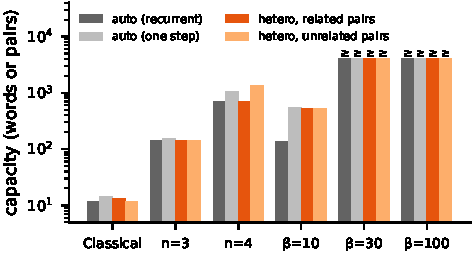
\includegraphics[width=\figsize]{fig5_words.pdf}
\caption{E3, words ($N=512$, 20\% noise): capacity for auto-association (recurrent and one-step) and hetero-association with related and unrelated pairs. $\ge$: never failed up to $K=4096$.}
\label{fig:words}
\end{figure}
Word codes are correlated, so the classical network holds only 12 words ($0.02N$), far below $0.14N$ (Fig.~\ref{fig:words}). With one update, hetero-association is \emph{not} harder than auto-association for any model; for dense $n=4$, \emph{unrelated} pairs were the easiest task (capacity 1371 vs 1040 for one-step auto) while \emph{related} pairs were hardest (702). Running the auto-associative dynamics to convergence did not help: the recurrent capacity was equal to or below the one-step capacity for every model, and for the blunt modern network ($\beta=10$) iterating destroyed recall above 138 words while one step still worked. Modern networks with $\beta\ge30$ never failed in any task up to $K=4096$.

\subsection{DRM false memories (Q2)}
\begin{figure*}[t]
\centering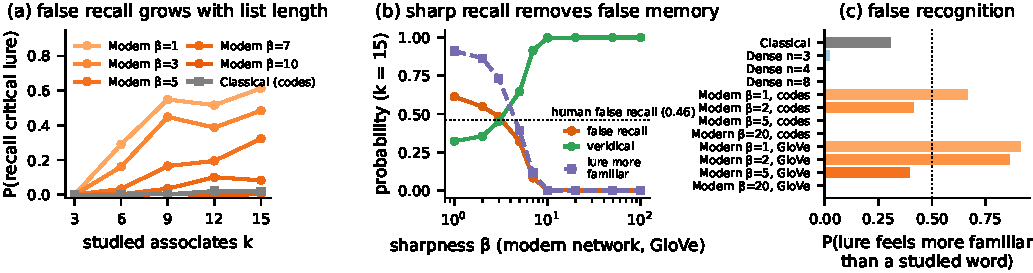
\includegraphics[width=\textwidth]{fig6_drm.pdf}
\caption{E4, DRM. (a) Probability that free recall produces the unstudied lure, vs number of studied associates. (b) Effect of sharpness at $k=15$ (modern network on GloVe vectors): false recall, veridical recall, and probability that the lure is more familiar than a studied word; dotted: human mean false recall~\cite{stadler99}. (c) Probability that the lure is more familiar ($-E$) than a studied word.}
\label{fig:drm}
\end{figure*}
In GloVe space the lure is the closest word of the whole lexicon to the average of its list for 19/31 lists, so a network that \emph{blends} the list should ``remember'' the lure. This is what the modern network does at low $\beta$ (Fig.~\ref{fig:drm}a): false recall rises with list length (for $\beta=3$: 0, 0.16, 0.45, 0.39, 0.48 for $k=3,\ldots,15$), reproducing the list-length effect of Robinson \& Roediger~\cite{robinson97}. At $\beta=3$ mean false recall (0.48) matches the human mean (0.46~\cite{stadler99}). Increasing $\beta$ trades false memory for veridical recall, with a sharp transition between $\beta=5$ and 10, beyond which the lure is never recalled (Fig.~\ref{fig:drm}b). Recognition shows the same dial: at $\beta=1$ the lure is more familiar than 91\% of the studied words, at $\beta\ge10$ than none. The classical network shows weak false recall (0.02 at $k=15$) and moderate false recognition (0.31); dense networks show none. On binary codes the modern network produced much less false recall (0.23 at $\beta=1$), because hashing distorts the geometry of the centroid (the lure is closest to the code centroid in only 5/31 lists). Per list, the model is all-or-none: it falsely recalls \emph{window} (human 0.65) but also \emph{king} (human 0.10, the lowest~\cite{stadler99}) and never \emph{cup}, whose GloVe neighbours are about sport (\emph{world cup}).

\section{Discussion and Conclusion}
\textbf{Q1.} The three published capacity results reproduce, but the ``exponential'' capacity of modern networks is capacity per feature neuron: each memory needs its own hidden neuron and $N$ synapses, so at equal synaptic cost the gain over the classical network is a constant factor of $\approx$4. On realistic, correlated data the decisive variable is sharpness: the classical network failed with 10 digits, while $\beta\ge300$ matched a perfect nearest-neighbour lookup; and too small a $\beta$ caps capacity whatever the network size.

\textbf{Q2.} Sharpness controls the kind of error. Blunt models make blends (spurious ``average'' states); sharp models make mix-ups with real, similar memories. In the DRM task a blending network reproduces three human findings: false recall of the lure at roughly the human rate, its growth with list length, and lure familiarity comparable to studied words. A sharp network removes false memory entirely. Humans thus behave like a moderately blunt memory, which trades exact recall for gist, consistent with global-matching accounts~\cite{arndt98}. The model does not capture list-to-list variability (king), which depends on associative norms~\cite{roediger95} rather than co-occurrence statistics.

\textbf{Q3.} My prediction that hetero-association hurts the classical network more was wrong. Within the similarity--separation--projection framework~\cite{millidge22} hetero-association only changes the projection; when partners are unrelated it \emph{decorrelates} the output space, so crosstalk from similar cues lands on unrelated targets and partly cancels. Related pairs restore the correlation and the interference. Recurrence did not help either: with correlated memories, iterating pulls the state into blends.

\textbf{Novelty.} (i) One controlled comparison of classical, dense and modern networks along a single sharpness dial, on identical memories and cues across random, image and word data; (ii) a synapse-matched comparison showing the modern advantage is a constant factor; (iii) the observation that blunt $\beta$ caps capacity independently of $N$; (iv) a modern-Hopfield account of DRM false recall and recognition with list-length and sharpness effects; (v) evidence that unrelated hetero-association is easier than auto-association on semantic data. \textbf{Limitations.} Binary word codes distort semantic geometry; the DRM recall readout is deterministic per list; free recall is modelled as independent random starts rather than a sequential search; sizes are small ($N\le784$).

\textbf{Reproduced vs new.} Reproduced: the $0.14N$ limit~\cite{ags85}, $N^{n-1}$ scaling~\cite{krotov16}, exponential/one-step retrieval~\cite{ramsauer21}. Everything else is new. All models were implemented from the papers' equations in NumPy; the authors' repositories~\cite{krotov16,ramsauer21} were not used.

\section*{Code, Data and Reproducibility}
Code, results and a live demo: \url{https://github.com/GrandsonOfBuddha/modern-hopfield-memory}. \texttt{run\_all.sh} regenerates every number and figure ($\approx$40\,min on a laptop); MNIST and GloVe are downloaded automatically, and the 20\,000-word GloVe subset is included. The models have no trained weights: the stored patterns \emph{are} the weights and are regenerated from fixed random seeds.

\section*{Individual Contribution}
This was a single-member project with no group partner; Soham Chatterjee is responsible for all components (study design, experiments, analysis, report and slides).

\begin{thebibliography}{99}
\footnotesize
\bibitem{hopfield82} J.~J.~Hopfield, ``Neural networks and physical systems with emergent collective computational abilities,'' \emph{PNAS}, vol.~79, no.~8, pp.~2554--2558, 1982.
\bibitem{ags85} D.~J.~Amit, H.~Gutfreund, and H.~Sompolinsky, ``Storing infinite numbers of patterns in a spin-glass model of neural networks,'' \emph{Phys.\ Rev.\ Lett.}, vol.~55, no.~14, pp.~1530--1533, 1985.
\bibitem{krotov16} D.~Krotov and J.~J.~Hopfield, ``Dense associative memory for pattern recognition,'' in \emph{Proc.\ NeurIPS}, vol.~29, 2016.
\bibitem{demircigil17} M.~Demircigil, J.~Heusel, M.~L\"owe, S.~Upgang, and F.~Vermet, ``On a model of associative memory with huge storage capacity,'' \emph{J.\ Stat.\ Phys.}, vol.~168, pp.~288--299, 2017.
\bibitem{ramsauer21} H.~Ramsauer \emph{et al.}, ``Hopfield networks is all you need,'' in \emph{Proc.\ ICLR}, 2021.
\bibitem{krotov21} D.~Krotov and J.~J.~Hopfield, ``Large associative memory problem in neurobiology and machine learning,'' in \emph{Proc.\ ICLR}, 2021.
\bibitem{millidge22} B.~Millidge, T.~Salvatori, Y.~Song, T.~Lukasiewicz, and R.~Bogacz, ``Universal Hopfield networks: A general framework for single-shot associative memory models,'' in \emph{Proc.\ ICML}, PMLR 162, pp.~15561--15583, 2022.
\bibitem{lecun98} Y.~LeCun, L.~Bottou, Y.~Bengio, and P.~Haffner, ``Gradient-based learning applied to document recognition,'' \emph{Proc.\ IEEE}, vol.~86, no.~11, pp.~2278--2324, 1998.
\bibitem{pennington14} J.~Pennington, R.~Socher, and C.~D.~Manning, ``GloVe: Global vectors for word representation,'' in \emph{Proc.\ EMNLP}, pp.~1532--1543, 2014.
\bibitem{charikar02} M.~S.~Charikar, ``Similarity estimation techniques from rounding algorithms,'' in \emph{Proc.\ STOC}, pp.~380--388, 2002.
\bibitem{roediger95} H.~L.~Roediger and K.~B.~McDermott, ``Creating false memories: Remembering words not presented in lists,'' \emph{J.\ Exp.\ Psychol.: Learn., Mem., Cogn.}, vol.~21, no.~4, pp.~803--814, 1995.
\bibitem{robinson97} K.~J.~Robinson and H.~L.~Roediger, ``Associative processes in false recall and false recognition,'' \emph{Psychol.\ Sci.}, vol.~8, no.~3, pp.~231--237, 1997.
\bibitem{stadler99} M.~A.~Stadler, H.~L.~Roediger, and K.~B.~McDermott, ``Norms for word lists that create false memories,'' \emph{Mem.\ Cogn.}, vol.~27, no.~3, pp.~494--500, 1999.
\bibitem{arndt98} J.~Arndt and E.~Hirshman, ``True and false recognition in MINERVA2: Explanations from a global matching perspective,'' \emph{J.\ Mem.\ Lang.}, vol.~39, no.~3, pp.~371--391, 1998.
\bibitem{nelson04} D.~L.~Nelson, C.~L.~McEvoy, and T.~A.~Schreiber, ``The University of South Florida free association, rhyme, and word fragment norms,'' \emph{Behav.\ Res.\ Methods}, vol.~36, no.~3, pp.~402--407, 2004.
\end{thebibliography}

\end{document}
